\documentclass[11pt]{article}
\usepackage[margin=1in]{geometry}
\usepackage{graphicx}
\usepackage{booktabs}
\usepackage[hidelinks]{hyperref}
\usepackage{amsmath}
\usepackage{enumitem}

\title{Oracle-Anchored LVR Recapture with Selective Dutch Auction Repricing}
\author{Author name withheld for double-blind review}
\date{May 2026}

\begin{document}
\maketitle

\begin{abstract}
Liquidity providers in automated market makers lose value when a pool price is stale relative to a faster reference market. This adverse-selection cost is known as loss-versus-rebalancing (LVR). We study a Uniswap v4 hook that uses an external oracle to detect stale pool states, charges stale-price trades with a square-root fee rule derived from one-step LVR accounting, and optionally routes repricing through a Dutch auction. The main comparison is against other v4-hook designs on the same replay inputs: a base oracle-anchored hook without the auction path, a broad all-stale auction rule, and the proposed selective auction rule that opens only when the auction improves LP accounting relative to the base hook. On an observed-flow replay covering 54 multi-hour windows across seven Uniswap v3 pools (36 routine four-hour windows and 18 historical two-hour stress windows, roughly 180 hours of trading in total), the selective auction improves LP uplift versus the broad all-stale auction in 28 windows, leaves 26 unchanged, and worsens none. Its mean trigger rate is 0.9825\%, compared with 5.8233\% for the broad auction rule, while every triggered selective-auction window fills in the replay. A separate full-month October 2025 grid covering four pools, 89{,}220 swaps, and 8{,}784 oracle updates across 124 four-hour windows calibrates the auction layer and retains fixed-fee v3 only as a legacy leakage check.
\end{abstract}

\section{Introduction}
An automated market maker (AMM) quotes prices from its own on-chain state. If an external market moves first, the AMM can briefly quote a stale price. A fast arbitrageur can then trade against the stale pool, move the pool toward the external price, and capture value that would otherwise belong to liquidity providers (LPs). This paper studies that event at hook level: when a Uniswap v4 pool is stale, can a hook redirect stale-price value back to LPs without leaving the pool unrepriced?

The accounting object is loss-versus-rebalancing (LVR) [1]. LVR measures the value LPs lose relative to a continuously rebalanced inventory benchmark when they provide liquidity to an AMM. In this paper, we use LVR in a narrower execution sense: a one-step stale repricing trade creates a measurable stale-price loss for LPs before fees. A hook can then decide whether to charge the repricing trader directly, open a solver auction around that repricing right, or leave ordinary AMM execution unchanged.

The relevant design question is not whether this mechanism beats an old static-fee pool. Fixed-fee Uniswap v3 is useful as a legacy leakage reference, but it is not the right primary benchmark for a v4 hook. The real benchmark is a set of v4-hook alternatives:
\begin{itemize}[leftmargin=0.25in]
\item \textbf{Base oracle-anchored hook}: detects stale prices and charges the deterministic square-root hook fee, but has no Dutch auction path.
\item \textbf{Broad all-stale auction hook}: opens auctions for every stale/toxic opportunity after a solver-cost reserve.
\item \textbf{Selective auction hook}: opens an auction only when it improves LP accounting relative to the base hook fee.
\end{itemize}

The contribution is therefore threefold. First, we give a plain hook-level interpretation of stale-price LVR and derive the square-root fee that recovers the one-step stale loss in a constant-product pool. Second, we position the design against existing v4 hook patterns: dynamic-fee hooks, oracle hooks, and auction-managed AMM work. Third, we evaluate the incremental auction design against hook-level baselines, showing that the selective rule triggers less often than the broad auction rule while improving LP uplift relative to the base hook.

\section{Reader Guide and Definitions}
This section defines the terms used throughout the paper before introducing the formulas.

\begin{description}[leftmargin=0.35in, style=nextline]
\item[AMM.]
An automated market maker is an on-chain exchange where smart-contract state determines the swap price. Uniswap v3 and v4 pools are AMMs.

\item[LP.]
A liquidity provider deposits assets into a pool. In return, the LP earns fees but bears inventory and adverse-selection risk.

\item[Hook.]
In Uniswap v4, a hook is an external smart contract attached to a pool. It can run before or after pool actions such as swaps and liquidity changes. Hooks are the v4 mechanism for pool-specific custom logic.

\item[Dynamic fee.]
A v4 dynamic fee is a swap fee that can change over time or per swap. A \texttt{beforeSwap} hook can return a fee override in a dynamic-fee pool.

\item[Oracle.]
An oracle is a reference price source. This paper uses Chainlink as the primary reference and treats Pyth, Binance, and deep-pool references as sensitivity inputs.

\item[Stale price.]
A pool is stale when its current pool price differs materially from the reference price. The paper measures this through a pool-oracle stale gap.

\item[LVR.]
Loss-versus-rebalancing is the adverse-selection cost LPs pay when AMM inventory is rebalanced at stale prices rather than continuously marked to a reference market.

\item[Toxic flow.]
In this paper, toxic flow means informed stale-price repricing flow. It is toxic because it trades against a stale quote and creates LP loss before fees.

\item[Solver.]
A solver is an actor that can fill a repricing auction. The solver receives a concession from the stale-price value and LPs receive the rest.

\item[Dutch auction.]
A Dutch auction starts with a low solver concession and increases it over time until a solver clears, the auction expires, or a reserve/cap blocks execution.

\item[LP net.]
LP net is fee revenue minus gross stale LVR. Positive LP net means fees more than cover the modeled stale-price loss.

\item[LP uplift vs base hook.]
LP uplift versus the base hook is the incremental LP net created by an auction rule relative to the deterministic hook-only fee path.
\end{description}

\section{Related Work and Positioning}
This paper piggybacks on three existing strands of work.

First, the LVR literature gives the economic accounting. Milionis, Moallemi, Roughgarden, and Zhang define LVR as an AMM adverse-selection cost relative to a continuously rebalanced benchmark [1]. We do not build a continuous-time AMM model. We use the LVR framing to price a single stale repricing event and then ask how a v4 hook should respond to that event.

Second, Uniswap v3 and v4 provide the market structure. Uniswap v3 introduced concentrated liquidity, which makes liquidity more capital efficient but also makes position shape important [2]. Uniswap v4 keeps concentrated liquidity and adds hooks, singleton accounting, and more flexible fee logic [3]. Official v4 documentation describes hooks as pool-attached contracts that can customize behavior around swap and liquidity lifecycle points [4], and describes dynamic fees as a v4 mechanism that can adjust fees per swap through \texttt{beforeSwap} [5]. Our hook is therefore not a new AMM; it is a v4 customization of swap pricing and liquidity admission.

Third, auction and hook designs provide the comparison class. The am-AMM paper studies auction-managed AMMs where the auction sells broader AMM control rights [8]. Frequent batch auction work motivates auctions as a response to speed races [9]. Existing v4 hook examples show that hooks can implement specialized execution and oracle logic: TWAMM hooks split large orders over time [6], truncated oracle hooks smooth oracle movements [7], and dynamic-fee hooks adjust swap fees [5]. Our mechanism is narrower than am-AMM governance and narrower than generic dynamic fees. It sells a short-lived stale-repricing right only when the hook counterfactual leaves LPs worse off.

\begin{center}
\begin{tabular}{p{0.25\textwidth}p{0.30\textwidth}p{0.32\textwidth}}
\toprule
Design family & What it controls & Difference from this paper \\
\midrule
Fixed-fee AMM & Static fee tier & Legacy reference only; cannot distinguish stale repricing flow from ordinary flow. \\
Generic dynamic-fee hook & Fee level as a function of volatility, volume, source, or other state & Our fee is tied to one-step stale-loss accounting, not a heuristic. \\
Oracle hook & Reference-price or oracle update behavior & Our oracle gap triggers repricing protection rather than publishing an oracle alone. \\
TWAMM hook & Time-sliced large-order execution & Our auction concerns stale repricing rights, not long-horizon user order slicing. \\
am-AMM / auction-managed AMM & Broader auctioned AMM control rights & Our auction is local and conditional: one stale state, one short-lived repricing opportunity. \\
\bottomrule
\end{tabular}
\end{center}

\section{Mechanism Overview}
The proposed hook has three pieces.

The first piece is the \textbf{base hook fee}. When the oracle and pool disagree, the hook computes an exact premium from the square-root ratio between the oracle price and the pool price. The deterministic fee is
\[
\texttt{hookFee} = \texttt{baseFee} + \alpha \cdot \texttt{exactPremium},
\]
subject to \texttt{maxFee}. This is the hook-only counterfactual used as the main benchmark.

The second piece is the \textbf{stale-gap trigger}. The unsigned gap is
\[
\texttt{stale\_gap\_bps\_before}
= \left|\log(\texttt{oracle\_mid}/\texttt{pool\_mid})\right| \times 10{,}000.
\]
An auction can open only when
\[
\texttt{stale\_gap\_bps\_before} \geq \texttt{trigger\_gap\_bps}.
\]
The sign is stored separately. A positive sign means the oracle is above the pool, so the pool is stale low.

The third piece is the \textbf{selective Dutch auction}. The broad auction rule opens too often because it auctions any stale/toxic opportunity after a solver-cost reserve. The selective rule instead asks whether the auction improves LP net relative to the base hook. If the base hook already protects LPs, the auction does not open. If the base hook leaves LPs exposed, the auction starts with a small solver concession and increases that concession until a solver clears or the reserve/cap blocks the fill.

\section{Fee Formula}
The square-root fee is an accounting reserve for stale repricing, not an arbitrary fee knob. Let the pool mid be \(P\) and the reference mid be \(P' = P e^z\), where \(z\) is the signed log gap. For a constant-product pool with invariant \(xy=L^2\), the pool state aligned with price \(P\) is
\[
x(P) = \frac{L}{\sqrt{P}},
\qquad
y(P) = L\sqrt{P}.
\]
For a one-step repricing from \(P\) to \(P'\), the exact fee fraction on the informed input that recovers stale-price loss is
\[
f^\star(z) = e^{|z|/2} - 1.
\]

\subsection{Intuitive geometric-mean proof}
The easiest way to see the formula is through the AMM's average execution price. A constant-product pool does not reprice from \(P\) to \(P'\) at either endpoint price. The average execution price over the full repricing trade is the geometric mean:
\[
\bar P = \sqrt{P P'}.
\]
This follows directly from the reserve changes. If the pool starts at price \(P=y/x\) and ends at \(P'\), the quote paid divided by base received over the constant-product path equals \(\sqrt{PP'}\).

Now consider \(P'>P\), meaning the oracle is above the pool and the pool is stale low. The informed trader buys base from the pool at average price \(\bar P\), while that base is worth \(P'\) at the reference market. The stale value extracted per unit of quote paid is therefore
\[
\frac{P' - \bar P}{\bar P}
=
\frac{P'}{\sqrt{P P'}} - 1
=
\sqrt{\frac{P'}{P}} - 1.
\]
This is the required fee fraction on the quote input if the hook wants to recover the one-step stale loss.

The other direction is symmetric. If \(P'<P\), the pool is stale high. The informed trader sells base into the pool at average price \(\bar P\), while that base is worth only \(P'\) at the reference market. The stale value extracted per unit of base input, valued at \(P'\), is
\[
\frac{\bar P - P'}{P'}
=
\frac{\sqrt{P P'}}{P'} - 1
=
\sqrt{\frac{P}{P'}} - 1.
\]
Both directions therefore reduce to
\[
f^\star
=
\sqrt{\frac{\max(P,P')}{\min(P,P')}} - 1
=
e^{|z|/2}-1,
\]
where \(z=\log(P'/P)\). Locally,
\[
f^\star(z) = \frac{|z|}{2} + O(z^2),
\]
so the familiar half-gap rule is the first-order approximation.

Written in oracle and pool mids, the exact premium is
\[
\texttt{exactPremium} =
\begin{cases}
\sqrt{\texttt{oracle\_mid}/\texttt{pool\_mid}} - 1, & \text{oracle above pool},\\
\sqrt{\texttt{pool\_mid}/\texttt{oracle\_mid}} - 1, & \text{oracle below pool}.
\end{cases}
\]
The Dutch auction does not replace this formula. It uses the base-hook fee path as the reserve/counterfactual that the auction must improve.

\section{Liquidity-Width Guard}
A swap fee controls what happens when stale flow arrives. It does not control how much fragile liquidity is exposed before the stale flow arrives. The implemented hook therefore also has a liquidity-width and centering guard for incoming LP positions.

The reason is specific to concentrated liquidity. Narrower ranges can multiply stale loss per dollar of position value. For a centered range \([P_a,P_b]\), define total log width \(W=\log(P_b/P_a)\) and center \(P_0=\sqrt{P_aP_b}\). At the center, the position value is
\[
V(P_0)=2L\sqrt{P_0}(1-e^{-W/4}).
\]
The normalized gross-LVR rate at the center is amplified to
\[
\frac{\ell(\sigma,P_0)}{V(P_0)}
=
\frac{\sigma^2}{8(1-e^{-W/4})}.
\]
If the designer budgets gross LVR over an effective latency window \(\Delta\) at no more than \(\epsilon\) of position value, it suffices to require
\[
\frac{\sigma^2\Delta}{8(1-e^{-W/4})} \leq \epsilon,
\qquad
W \geq W_{\min}
= -4\log\left(1-\frac{\sigma^2\Delta}{8\epsilon}\right).
\]
The October auction grid does not empirically validate LP repositioning behavior. The guard is included to show that the hook design addresses both sides of the stale-flow problem: \texttt{beforeSwap} prices stale repricing flow, while \texttt{beforeAddLiquidity} rejects marginal ranges that exceed the configured LVR budget.

\section{Empirical Design}
The evidence has two layers.

\subsection{Data and Replay Construction}
The historical input is Ethereum mainnet swap and \texttt{Sync} event data from Uniswap v3 pools. The replay reconstructs v3 pool state block by block, classifies each swap as informed or uninformed under the stale-gap rule defined in Section~3, and then re-prices the same observed flow through (a) the unmodified v3 fee tier, (b) the base oracle-anchored hook, (c) the broad all-stale auction overlay, and (d) the selective auction overlay. Reference prices come from Chainlink USD and ETH feeds for the relevant tokens; Pyth, Binance, and deep-pool references are reserved for sensitivity checks and are not used in the headline numbers.

The observed-flow replay covers 54 windows across seven Uniswap v3 pools, with 36 routine four-hour windows and 18 historical two-hour stress windows, totalling roughly 180 hours of trading. A \textbf{window} is a contiguous block range — four hours for routine windows and two hours for stress windows — over which informed/uninformed classification, fee accounting, and auction overlays are evaluated on the same swap stream. \textbf{Routine} windows are sampled from ordinary trading periods; \textbf{stress} windows are sampled from periods with larger oracle-pool dislocation, oracle disagreement, high activity, or known replay edge cases, and are flagged in the replay configuration rather than detected ex post. The October 2025 calibration grid is a separate full-month four-pool artifact covering WETH/USDC, WBTC/USDC, LINK/WETH, and UNI/WETH — 124 four-hour windows (31 per pool), 89{,}220 swap samples, and 8{,}784 oracle updates — and is used only to pick auction-layer parameters around the base hook fee law.

\subsection{Primary Benchmark: V4 Hook Ablation}
The primary benchmark is the observed-flow replay. It reconstructs v3 pool state, classifies observed swaps as informed or uninformed under the replay labels, replays fixed, hook, linear, and log fee policies, and overlays two auction policies on the same windows. This replay covers 54 windows across seven pools: 36 routine four-hour windows and 18 historical two-hour stress windows, totalling roughly 180 hours of trading.

The comparison is deliberately hook-native:
\begin{center}
\begin{tabular}{p{0.25\textwidth}p{0.28\textwidth}p{0.34\textwidth}}
\toprule
Benchmark & Trigger/reserve rule & Interpretation \\
\midrule
Base hook & No auction path & Oracle-anchored square-root fee only. This is the hook-without-auction counterfactual. \\
Broad all-stale auction & \texttt{all\_toxic} trigger, solver-cost reserve & Earlier/simple auction policy. It auctions more stale events. \\
Selective auction hook & \texttt{auction\_beats\_hook} trigger, \texttt{hook\_counterfactual} reserve & Proposed policy. It auctions only when LP accounting improves relative to the base hook. \\
\bottomrule
\end{tabular}
\end{center}

The reported LP columns are in each window's native quote units and should not be summed as one cross-pool dollar P\&L. The sign and direction are the relevant evidence.

\subsection{Parameter Calibration: October 2025 Grid}
The second layer is an October 2025 grid for four pools. It uses simulated correction trades on stale repricing opportunities and sweeps:
\begin{center}
\begin{tabular}{lr}
\toprule
Parameter & Values \\
\midrule
\texttt{trigger\_gap\_bps} & 5, 10, 25, 50 \\
\texttt{base\_fee\_bps} & 1, 5, 30 \\
\texttt{start\_concession\_bps} & 10, 30, 100 \\
\texttt{concession\_growth\_bps\_per\_sec} & 0.5, 1.0, 5.0 \\
\texttt{max\_fee\_bps} & 500, 2500, 5000 \\
\bottomrule
\end{tabular}
\end{center}
This grid has 1,296 pool-parameter rows and 40,176 window-parameter rows. It is used to pick an auction-layer candidate around the base hook fee law, not to claim final production market share.

\subsection{Legacy Reference: Fixed-Fee V3}
Fixed-fee v3 remains in the paper only as a legacy leakage check. It asks how much stale-price loss an ordinary production fee tier would recover from the same modeled stale repricing opportunities. That is useful context, but it is not the benchmark that establishes the incremental value of the proposed v4 hook design.

\section{Results}
\subsection{Hook-Level Benchmark Results}
The main result is that the selective auction improves the broad auction rule while preserving the base hook as a reserve. Across the 54-window observed-flow replay, the selective rule improves LP uplift versus the broad all-stale auction in 28 windows, leaves 26 unchanged, and worsens none.

\begin{center}
\begin{tabular}{lrrrrrr}
\toprule
Regime & Windows & Positive delta & Broad uplift & Selective uplift & Delta & 95\% CI for delta \\
\midrule
Overall & 54 & 28 & -2.8646 & 2.7735 & 5.6381 & [1.7364,\ 9.5666] \\
Normal & 36 & 18 & -2.2242 & 3.0039 & 5.2281 & [0.5103,\ 10.5484] \\
Stress & 18 & 10 & -4.1454 & 2.3127 & 6.4581 & [0.0000,\ 11.0710] \\
\bottomrule
\end{tabular}
\end{center}

The selective rule is also materially less intrusive. The broad all-stale rule triggers on 5.8233\% of observed replay opportunities on average. The selective rule triggers on 0.9825\%. Every selective-auction window with at least one trigger has a 1.0 fill rate, and the run records no oracle fail-closed events under the selective rule.

This is the core benchmark result. The proposed design does not merely add an auction to the hook. It adds a more selective auction gate that preserves the base hook counterfactual and avoids auctioning stale events where the deterministic hook fee already protects LPs.

\subsection{Auction Parameter Calibration}
The selected October 2025 parameter set is:
\[
(10,\ 5,\ 10,\ 0.5,\ 2500),
\]
in the order trigger gap, base fee, starting concession, concession growth, and max fee. The choice is not an unconstrained optimum. It is a conservative deployment candidate within the tested grid: 10 bps trigger gap, 5 bps base fee, 10 bps starting solver concession, 0.5 bps/sec concession growth, and 2500 bps max fee.

\begin{figure}[htbp]
\centering
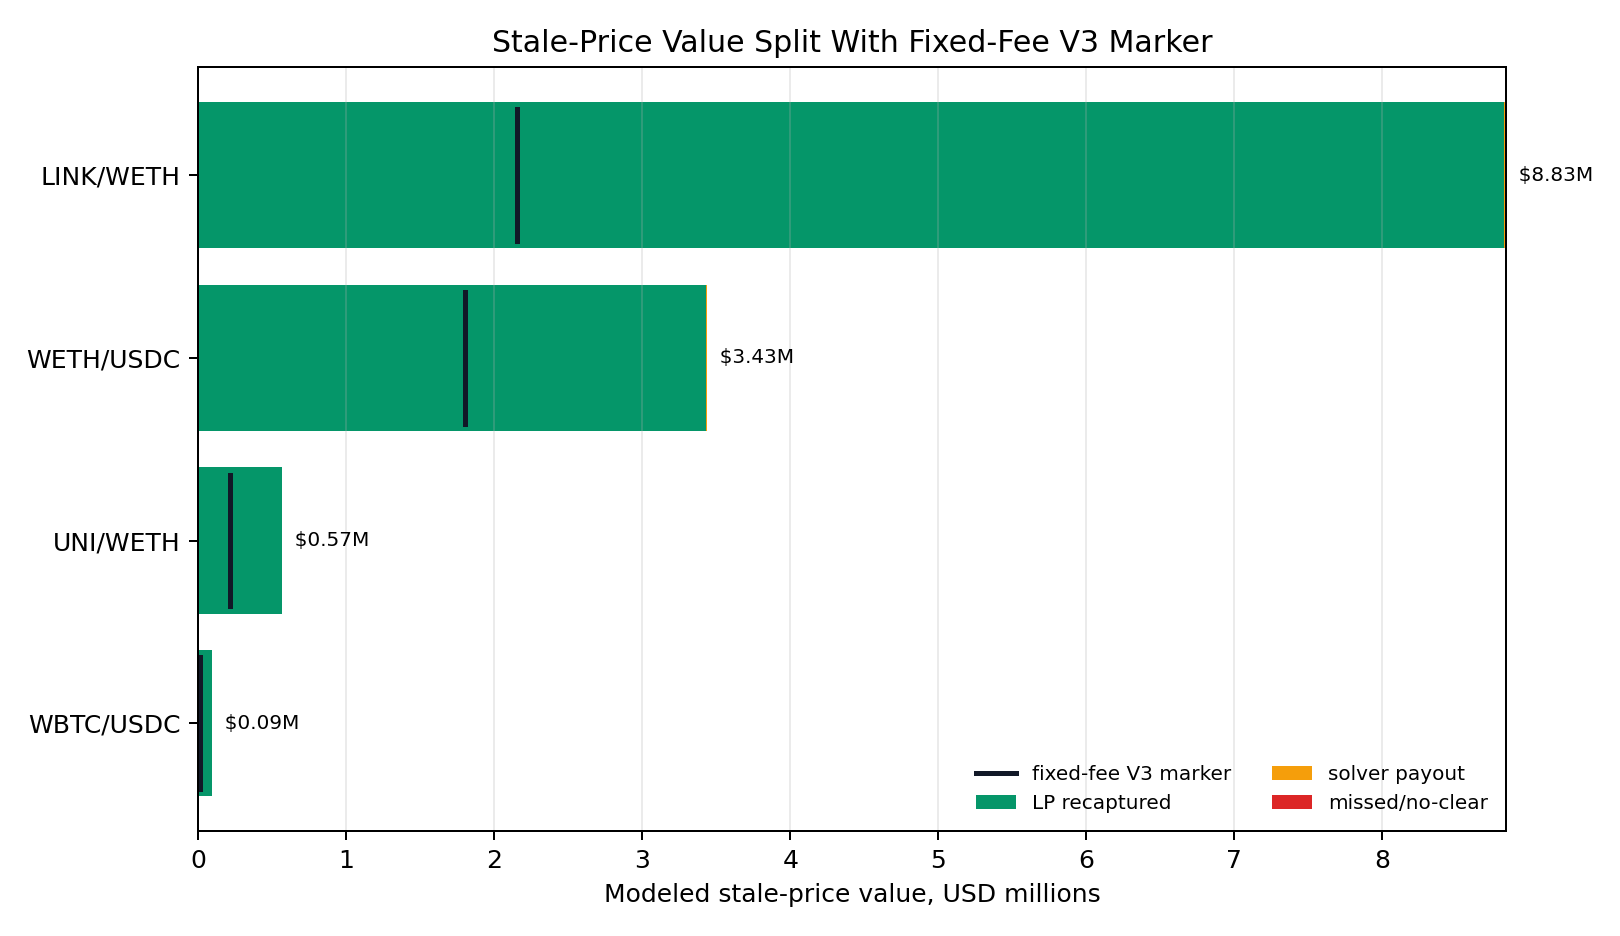
\includegraphics[width=0.92\textwidth]{reports/charts/chart_a_recapture_per_pool.png}
\caption{October 2025 calibration: USD-equivalent stale-price value split for the selected parameter set by pool. Green bars show LP-recovered stale value, orange shows solver payout, red shows missed/no-clear value, and the black marker shows the fixed-fee v3 legacy reference on the same modeled opportunities.}
\label{fig:recapture-pool-policy}
\end{figure}

\begin{center}
\begin{tabular}{lrrrrr}
\toprule
Pool & Recapture & Clear rate & Legacy v3 ref. & Triggers & Solver payout \\
\midrule
WETH/USDC & 99.9000\% & 1.0000 & 52.5709\% & 1242 & 10.0000 bps \\
WBTC/USDC & 99.9000\% & 1.0000 & 16.9001\% & 800 & 9.9995 bps \\
LINK/WETH & 99.9000\% & 1.0000 & 24.4175\% & 3163 & 10.0000 bps \\
UNI/WETH & 99.9000\% & 1.0000 & 37.7356\% & 2209 & 10.0000 bps \\
\bottomrule
\end{tabular}
\end{center}

The uniform 99.9\% recapture is a mechanical consequence of the selected auction concession, not a claim that all four pools have identical economics. The starting concession gives the solver 10 bps of gross stale-LVR value, not 10 bps of trade notional, so a quickly clearing auction leaves roughly 99.9\% of modeled stale LVR to LPs.

The solver economics are the main caveat:
\begin{center}
\begin{tabular}{lrrrr}
\toprule
Pool & Filled auctions & Stale value & Solver payout & Avg payout \\
\midrule
LINK/WETH & 3163 & \$8.83M & \$8.8k & \$2.79 \\
WETH/USDC & 1242 & \$3.43M & \$3.4k & \$2.77 \\
UNI/WETH & 2209 & \$565.1k & \$565.12 & \$0.26 \\
WBTC/USDC & 800 & \$92.7k & \$92.72 & \$0.12 \\
\midrule
Total & 7414 & \$12.93M & \$12.9k & \$1.74 \\
\bottomrule
\end{tabular}
\end{center}
The average payout is a break-even cost threshold. A solver must clear the auction below that cost, including gas and operational overhead, before the fill is profitable. This makes low-cost execution, batching, and multi-pool correction important future design requirements.

\subsection{Sensitivity}
\begin{figure}[htbp]
\centering
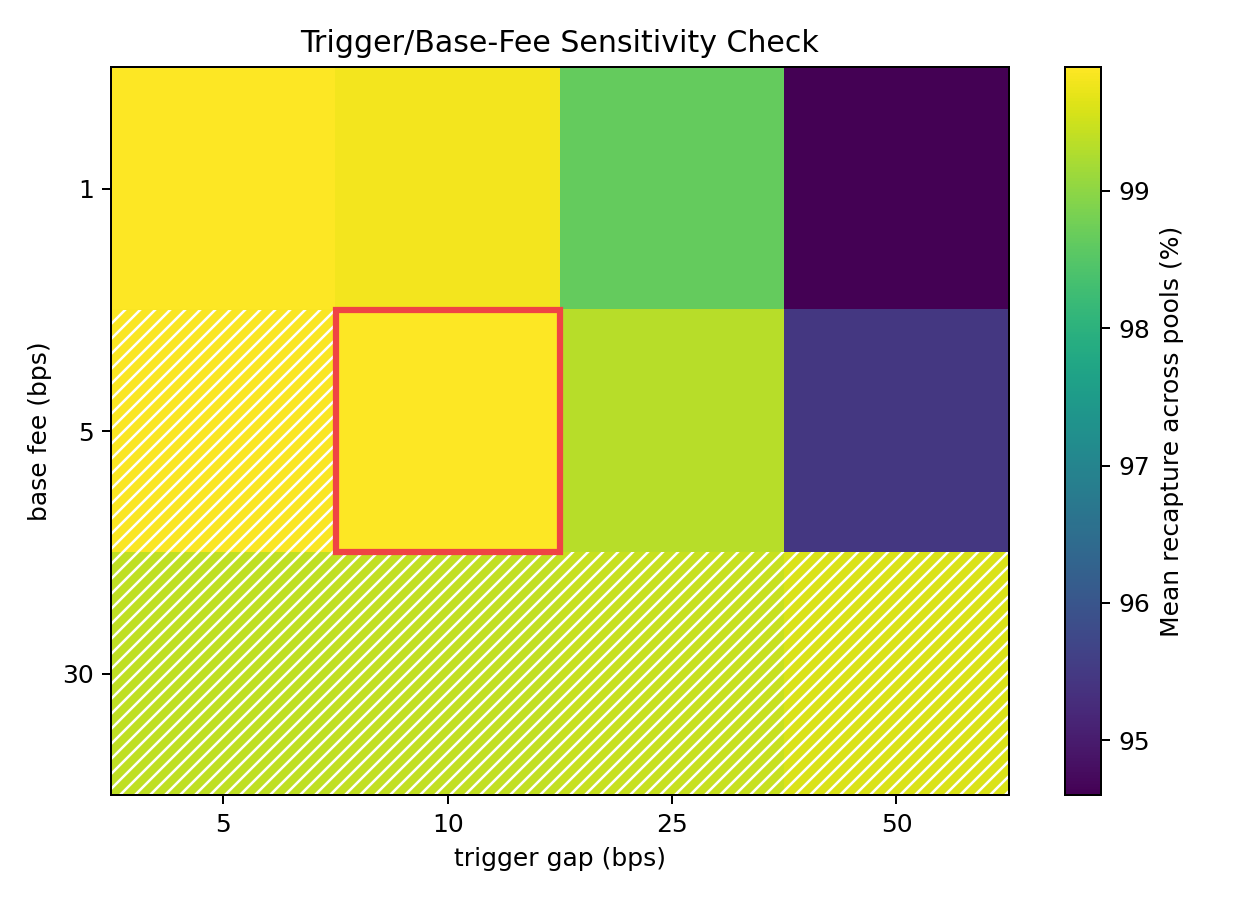
\includegraphics[width=0.78\textwidth]{reports/charts/chart_b_sensitivity_heatmap.png}
\caption{Trigger-gap by base-fee sensitivity check. The other auction parameters are fixed at the recommended values; hatched entries have at least one pool below 0.9 clear rate, and the red outline marks the recommended parameter set.}
\label{fig:sensitivity-heatmap}
\end{figure}

The largest one-step effect in the October grid is \texttt{base\_fee\_bps}: increasing the base fee lowers measured recapture because it removes marginal clears. The next-largest effects are starting concession and trigger gap. \texttt{max\_fee\_bps} and concession growth are second-order over this month slice.

\begin{center}
\begin{tabular}{lrrr}
\toprule
Parameter step & Mean delta & Std delta & Pools improved \\
\midrule
\texttt{base\_fee\_bps} up & -0.986049 pp & 0.562620 pp & 0/4 \\
\texttt{start\_concession\_bps} up & -0.699985 pp & 0.000013 pp & 0/4 \\
\texttt{trigger\_gap\_bps} up & -0.576773 pp & 0.424254 pp & 0/4 \\
\texttt{start\_concession\_bps} down & 0.199997 pp & 0.000004 pp & 4/4 \\
\bottomrule
\end{tabular}
\end{center}

\subsection{Legacy V3 Leakage Check}
The v3 fee tier is not the primary benchmark, but it remains useful to show the leakage that motivates a v4 mechanism. A static fee collects a percentage of trade notional; stale LVR is measured against the stale repricing opportunity. The two are not the same object.

\begin{center}
\begin{tabular}{lrrrr}
\toprule
Pool & V3 fee & V3 recapture & Implied stale loss & Gap to selected rule \\
\midrule
WETH/USDC & 30 bps & 52.5709\% & 57.07 bps & 47.3291 pp \\
WBTC/USDC & 5 bps & 16.9001\% & 29.59 bps & 82.9999 pp \\
LINK/WETH & 30 bps & 24.4175\% & 122.86 bps & 75.4825 pp \\
UNI/WETH & 30 bps & 37.7356\% & 79.50 bps & 62.1644 pp \\
\bottomrule
\end{tabular}
\end{center}
This table should be read as motivation, not as proof of superiority over v4 hook designs. The proof-of-design comparison is the hook ablation above.

\section{Discussion}
The revised evidence supports a more precise story than the earlier draft. The base oracle-anchored hook supplies the stale-loss fee floor. The broad auction rule shows what happens when auction logic is added too aggressively. The selective Dutch auction is better because it treats the base hook as a counterfactual reserve: it acts only where the auction can improve LP accounting.

This matters for an external audience because the mechanism has two goals that can conflict. LPs want stale-price value recovered, but traders and solvers need reliable execution. A hook that simply charges very high stale-flow fees can look good in LP accounting while failing to clear. An auction that triggers too often can add complexity where the base hook already works. The proposed design is therefore a selective execution layer around the fee formula, not a replacement for the fee formula.

The 10 bps trigger should be read as a deployment hypothesis. In the October grid, a 5 bps trigger opens more auctions on marginal stale states. Those states still often beat the legacy fixed-fee reference, but they clear less robustly. The 10 bps trigger is more selective and maintains clear rate across the four tested pools.

The solver economics remain unresolved. The October calibration pays solvers about \$1.74 per filled auction on average before gas, with large variation across pools. That is enough to motivate an auction design, but not enough to prove a live solver market. Practical deployment needs batching, low-cost settlement, explicit gas modeling, and multiple-solvers tests.

\section{Limitations}
The study is a replay, not a live-market experiment. It omits realistic gas costs, competitive solver dynamics, and full routing response. The observed-flow replay adds historical swaps and hook-policy ablations, but it still does not decide whether each historical user swap would route to this pool, another v4 hook pool, a v3 pool, a centralized exchange, or no venue under the changed state. The October grid tests correction trades rather than a full pending-auction state machine. Chainlink is the primary reference oracle, with Pyth, Binance, and deep-pool references reserved for sensitivity checks. The grid does not sweep \texttt{alphaBps}. The liquidity-width guard is derived and implemented, but the auction grid does not test LP repositioning behavior or range-width effects on realized order flow.

\section{Future Work}
The next empirical step is a multi-month replay using the same hook-level benchmark hierarchy: base hook, broad all-stale auction, selective auction, and legacy fixed-fee reference. The next market-design step is a two-pool competitive-routing simulation where traders choose between a base hook pool and a selective-auction hook pool. The auction model should also add gas costs, solver profit margins, multiple solvers, oracle disagreement, batching, and explicit fallback behavior when no solver clears.

\section{Conclusion}
The proposed design is best understood as a selective v4 hook improvement rather than as a comparison to fixed-fee v3. The base hook prices stale repricing flow with a square-root LVR fee. The Dutch auction adds an execution path only when that path improves LP accounting relative to the base hook. On the observed-flow replay, the selective rule improves LP uplift versus the broad all-stale auction in 28 of 54 windows, leaves the remaining 26 unchanged, and worsens none, while reducing the mean trigger rate from 5.8233\% to 0.9825\%. The fixed-fee v3 comparison remains useful as a leakage check, but the core result is the improvement over existing v4 hook variants.

\clearpage
\section{Appendix: Cross-Pool Calibration Check}
\begin{figure}[htbp]
\centering
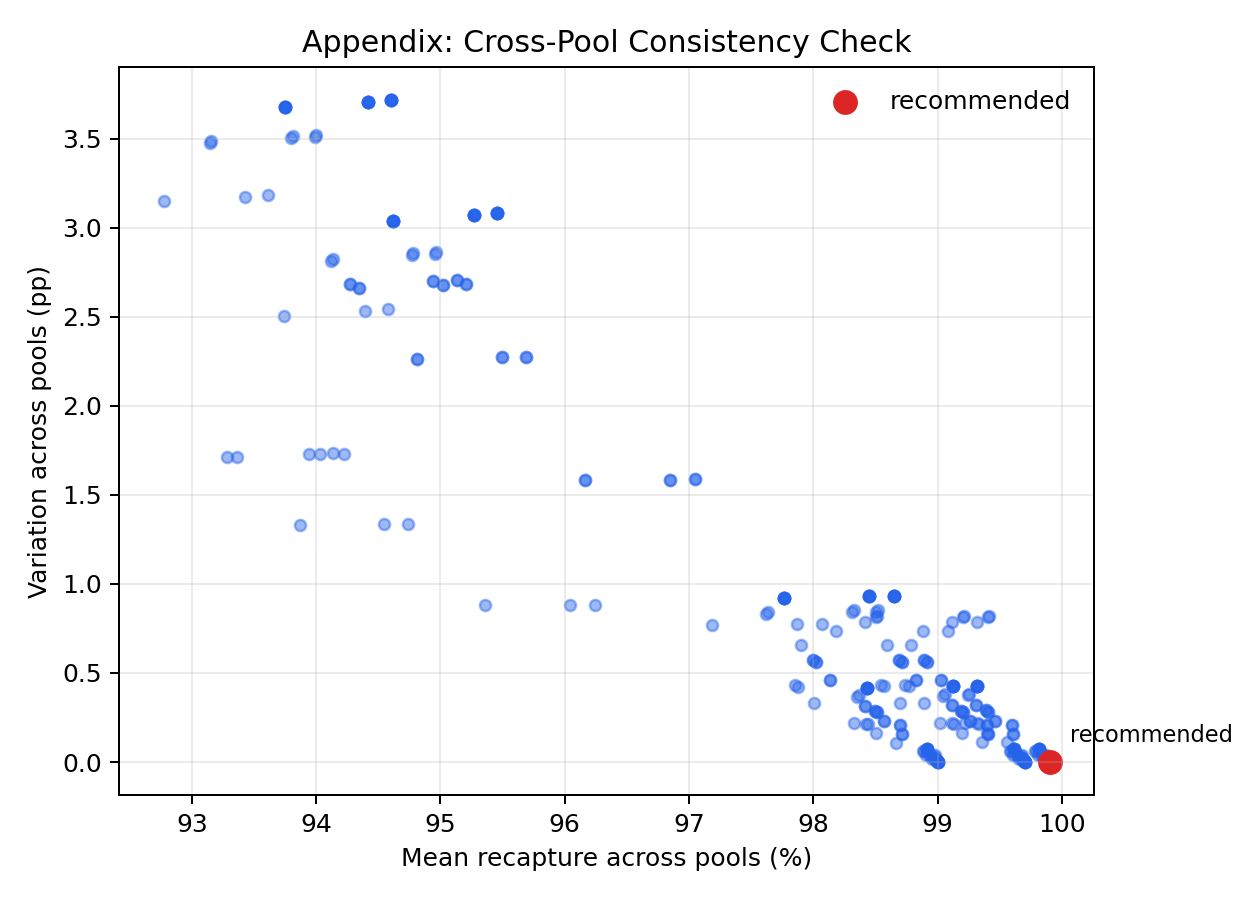
\includegraphics[width=0.78\textwidth]{reports/charts/chart_d_consistency.png}
\caption{Appendix check: cross-pool mean recapture versus variation across pools for every October 2025 parameter set.}
\label{fig:consistency}
\end{figure}

\section*{Code and Data Availability}
The Solidity hook implementation, replay engine, October 2025 calibration grid, and the figure-generation scripts are released as an open-source repository (URL withheld for double-blind review and to be provided on acceptance). The empirical results in this paper correspond to an immutable, version-tagged release of that repository. The observed-flow replay artifacts and the calibration grid CSVs live under \path{study_artifacts/} and \path{reports/} at that tag; the figures in this paper are regenerated from those artifacts by the scripts under \path{script/}.

\section*{Acknowledgments}
Acknowledgments are omitted for double-blind review and will be restored in the final version.

\clearpage
\section*{References}
\begin{enumerate}[leftmargin=0.25in]
\item Jason Milionis, Ciamac C. Moallemi, Tim Roughgarden, and Anthony Lee Zhang. ``Automated Market Making and Loss-Versus-Rebalancing.'' arXiv:2208.06046, August 2022, revised May 2024. DOI: 10.48550/arXiv.2208.06046.
\item Hayden Adams, Noah Zinsmeister, Moody Salem, River Keefer, and Dan Robinson. ``Uniswap v3 Core.'' Uniswap Labs whitepaper, March 2021. \href{https://uniswap.org/whitepaper-v3.pdf}{uniswap.org/whitepaper-v3.pdf}.
\item Hayden Adams, Moody Salem, Noah Zinsmeister, Sara Reynolds, Austin Adams, Will Pote, Mark Toda, Alice Henshaw, Emily Williams, and Dan Robinson. ``Uniswap v4 Core.'' Uniswap Labs whitepaper, August 2024. \href{https://app.uniswap.org/whitepaper-v4.pdf}{app.uniswap.org/whitepaper-v4.pdf}.
\item Uniswap Docs. ``Hooks.'' \href{https://developers.uniswap.org/docs/protocols/v4/concepts/hooks}{Uniswap v4 hooks documentation}.
\item Uniswap Docs. ``Dynamic Fees.'' \href{https://developers.uniswap.org/docs/protocols/v4/concepts/dynamic-fees}{Uniswap v4 dynamic-fees documentation}.
\item Uniswap Labs. ``Uniswap v4 TWAMM Hook.'' August 24, 2023. \href{https://blog.uniswap.org/v4-twamm-hook}{Uniswap Labs blog}.
\item Uniswap Labs. ``Uniswap v4 Truncated Oracle Hook.'' September 20, 2023. \href{https://blog.uniswap.org/uniswap-v4-truncated-oracle-hook}{Uniswap Labs blog}.
\item Austin Adams, Ciamac C. Moallemi, Sara Reynolds, and Dan Robinson. ``am-AMM: An Auction-Managed Automated Market Maker.'' arXiv:2403.03367, March 2024.
\item Eric Budish, Peter Cramton, and John Shim. ``The High-Frequency Trading Arms Race: Frequent Batch Auctions as a Market Design Response.'' \emph{The Quarterly Journal of Economics}, 130(4):1547--1621, 2015. DOI: 10.1093/qje/qjv027.
\end{enumerate}

\end{document}
